\documentclass[12pt, oneside]{article}
\usepackage[letterpaper, margin=1in]{geometry}
\usepackage[english]{babel}
\usepackage[utf8]{inputenc}
\usepackage{amsmath}
\usepackage{amsfonts}
\usepackage{amssymb}
\usepackage{tikz}
\usepackage{venndiagram}

\usepackage{fancyhdr}
\pagestyle{fancy}
\fancyhf{}
\rhead{Name: \hspace{1.5in} }
\lhead{BECA / Dr. Huson / 11.1 IB Math SL \\* 29 March 2018 \\* Test: Sequences \& series}

\vspace{1cm}

\renewcommand{\headrulewidth}{0pt}

\title{Worksheet and test template}
\author{Chris Huson}
\date{March 2018}

\begin{document}

\subsubsection*{\\* Answer on lined paper. Show work.}

\begin{enumerate}

\vspace{0.5 cm}

%\subsubsection*{Rational exponents and radicals}

\item In an arithmetic sequence, the first term is 7 and the second term is 11.
\begin{enumerate}
    \item Find the common difference.
    \item Find the eighth term.
    \item Find the sum of the first eight terms of the sequence.
\end{enumerate}

\item Given that for a geometric sequence $u_1=18$ and $u_3=8$
\begin{enumerate}
    \item Find the value of $r$.
    \item Given that $u_k$ is the first term of the sequence with a value less than one, find $k$.
    \item Find the sum of the infinite series $S_\infty$
\end{enumerate}

\item The first three terms of an arithmetic sequence are $u_1=5.1$, $u_2=5.5$, and $u_3=5.9$.
\begin{enumerate}
    \item Find the common difference.
    \item Given that the $k$th term of the sequence, $u_k=11.5$. Find $k$.
\end{enumerate}


\item Let $f(x) = 2x -3$ and $g(x)=(x-1)^2$
\begin{enumerate}
    \item Find $(f \circ g)(4)$
    \item Find $f^{-1}(x)$
\end{enumerate}


\item Simplify the expression $\sqrt{a} \cdot \sqrt{a^5}$

\item $(2x^2-2x-5)(x+3)-2x(x^2-x-4)$

\item What is the inverse of the function $y=\frac{2}{x+3}$?

\item Let $x=ln2$ and $y=ln5$. Write down the following expressions in terms of $x$ and $y$.
\begin{enumerate}
    \item $\ln \frac{2}{5}$
    \item $\ln 50$
    \item $\ln 0.1$
\end{enumerate}

\item Using the quadratic formula or otherwise, find the solution set to $2x^2-3x-5=0$.

\item Simplify the expression $2xi(4+3i)$.

\item Simplify the expression $\displaystyle \left( \frac{x^{-2}}{x^2} \right)^{\frac{1}{2}}$ to one with positive integer exponents and radicals.


%\item If $(x-2)$ is a factor of $f(x)=(x-2)(ax^2+bx+c)$, then what is the value of $f(2)$?

\newpage
\item The function $g$ is defined by graph of $y=g(x)$ below.
\begin{enumerate}
    \item Write down the equation for $g(x)$ in factored form.
    \item The function $h(x)$ is made by reflecting $g$ across the $y$-axis. What is the equation for $h(x)$?
\end{enumerate}

\begin{figure}[!ht]
    \centering
    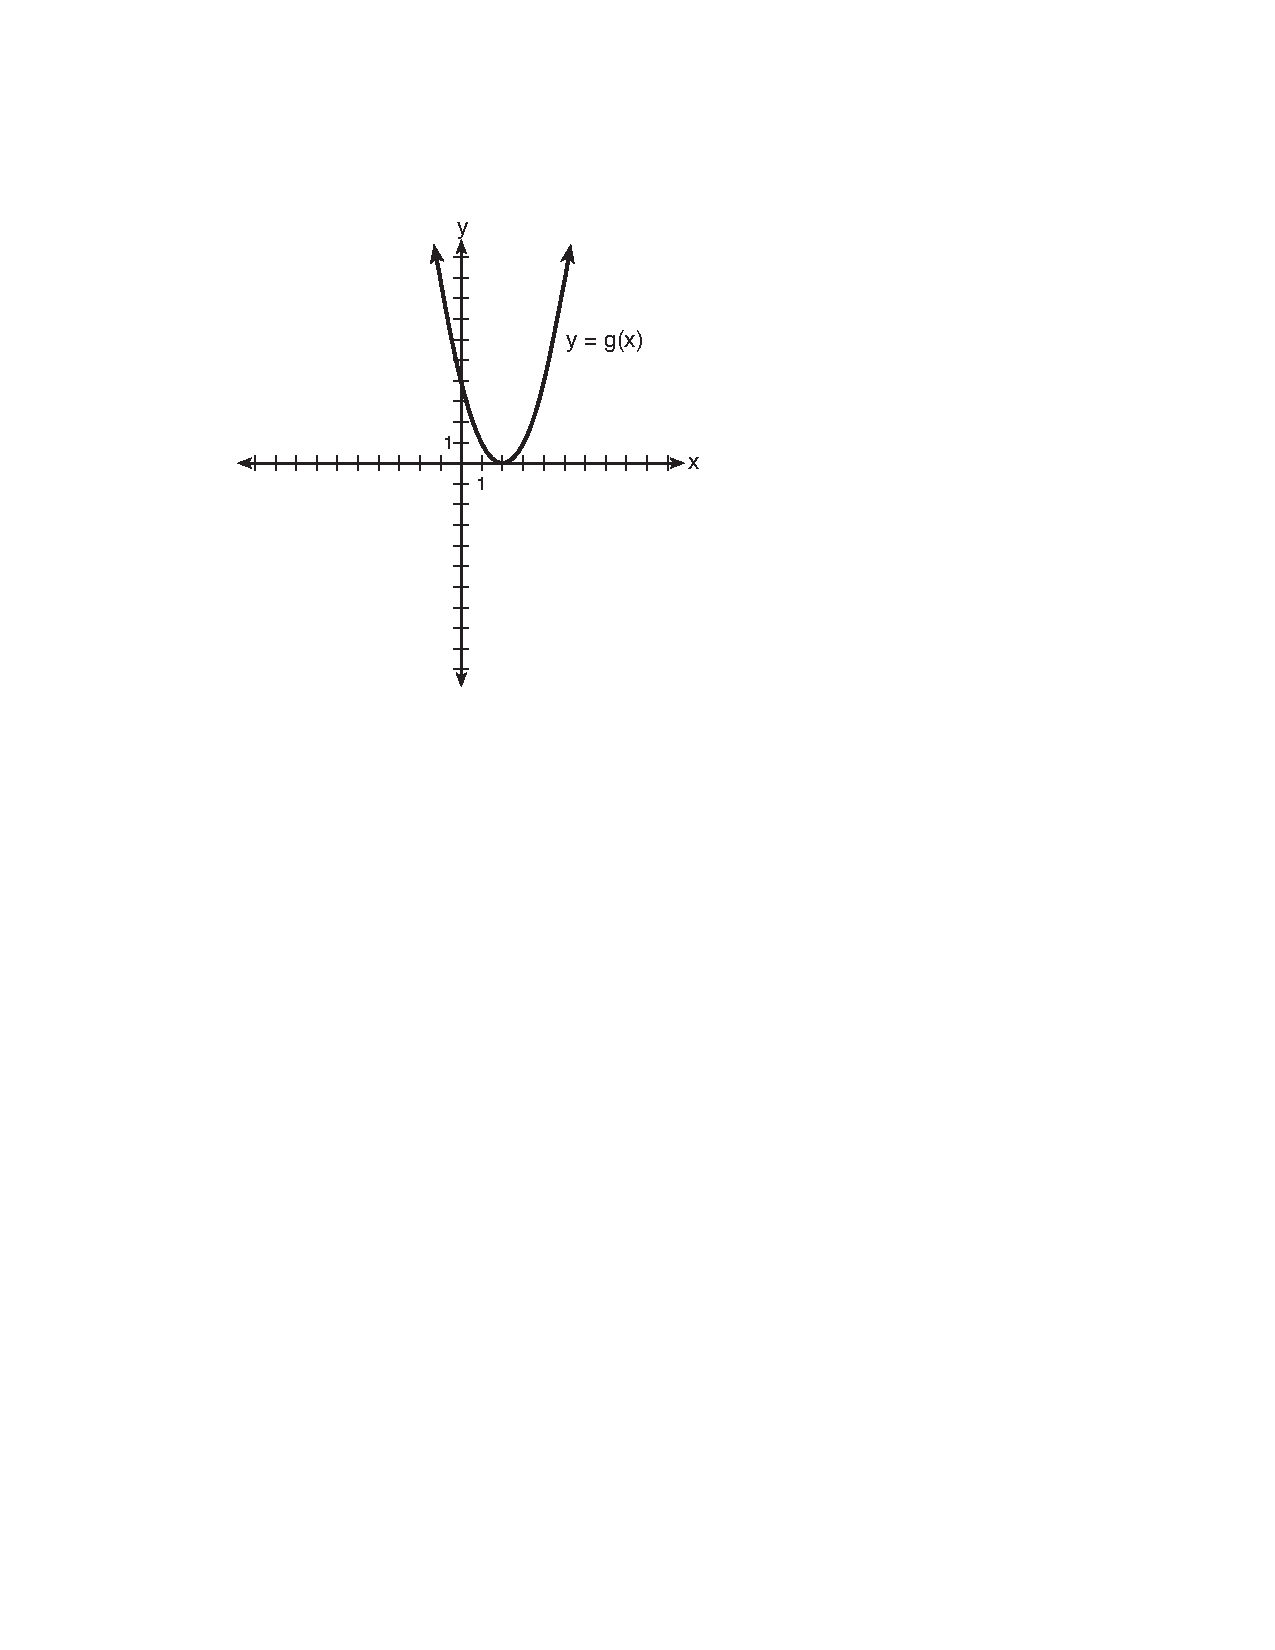
\includegraphics[width=0.4\textwidth]{parabola-graphic.pdf}
\end{figure}

\item Let $f(x) = x^2-6x+4$
\begin{enumerate}
    \item Rewrite quadratic in vertex form and state the vertex as an ordered pair.
    \item The parabola is translated vertically by $k$ units to make the function $g(x)$. The equation $g(x)=0$ has one solution. Find $k$.
\end{enumerate}

\item For each of the following questions select two applicable words from the following list: revenues, assets, premiums, costs, earnings, expenses, debt, reserves, overhead, investments.
\begin{enumerate}
    \item What financial measure would a business manager try to \emph{increase} in order to raise profits?
    \item What financial measure would a manager try to reduce to improve profitability?
    \item Since their customers could have large losses from a storm or other disaster at any time an insurance company maintains large amounts of what?
\end{enumerate}

\newpage
\subsubsection*{For these last two pages, answer in the space provided}

\item Graph $g(x)=30(1.5)^{\frac{x}{2}}-5$ on the set of axes below.
\begin{center}
    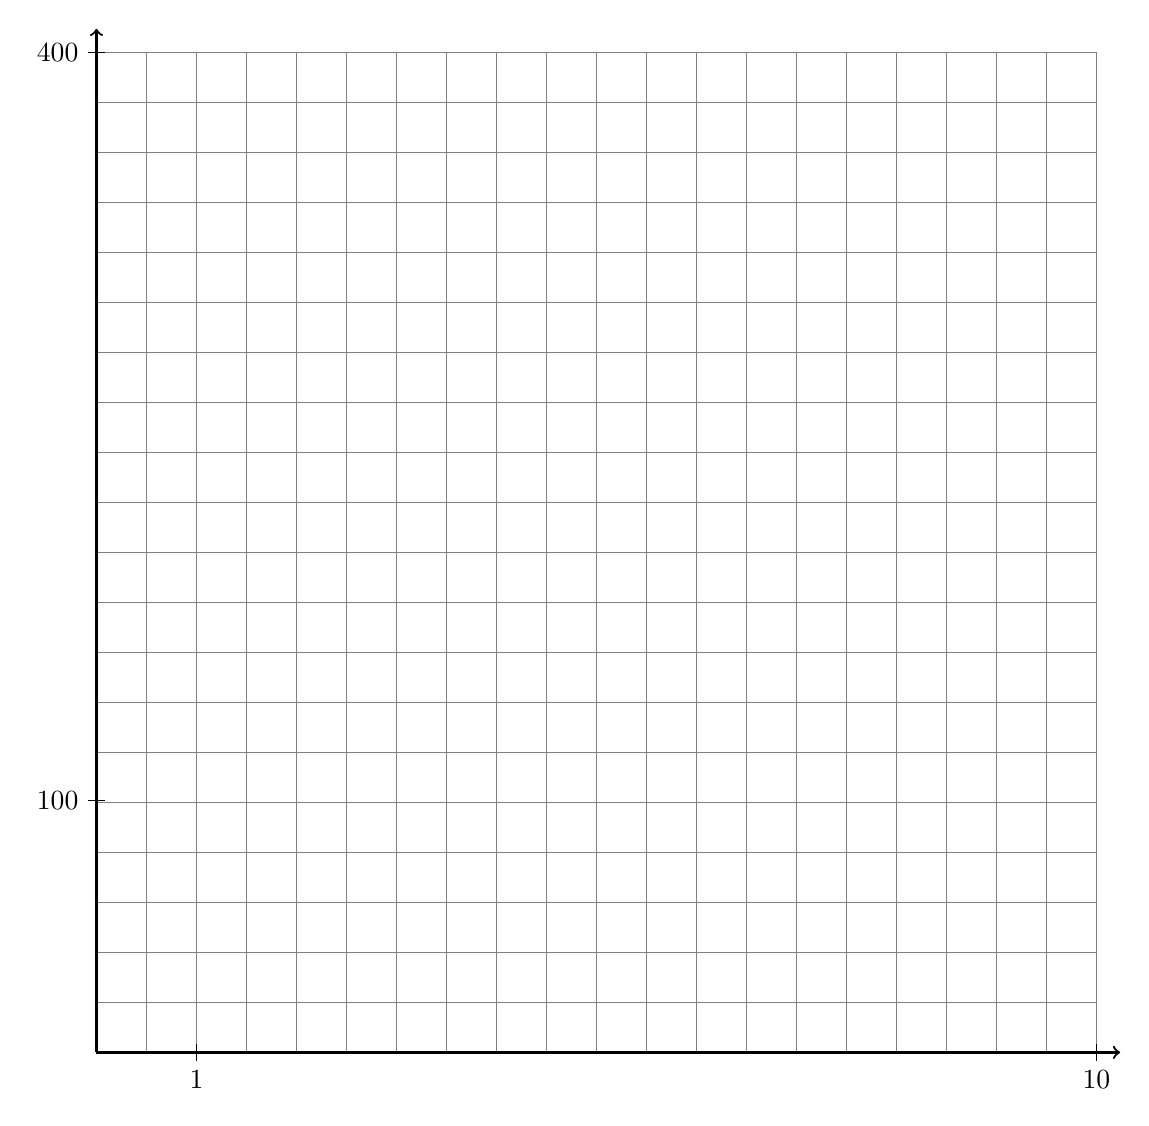
\begin{tikzpicture}
    \draw[step=0.25in,gray,very thin] (0,0) grid (12.7,12.7);
    \draw[thick,->] (0,0) -- (13,0); node[anchor=north west] {x};
    \draw[thick,->] (0,0) -- (0,13); node[anchor=south east] {y};
    \foreach \x in {1.27} \draw (\x cm,3pt) -- (\x cm,-3pt) node[anchor=north] {$1$};
    \foreach \x in {12.7} \draw (\x cm,3pt) -- (\x cm,-3pt) node[anchor=north] {10};
    \foreach \y in {3.2} \draw (3pt,\y cm) -- (-3pt,\y cm) node[anchor=east] {100};
    \foreach \y in {12.7} \draw (3pt,\y cm) -- (-3pt,\y cm) node[anchor=east] {400};
    \end{tikzpicture}
\end{center} %Alg2 Regents Jun2017
Is the function an example of exponential growth or exponential decay? Justify your answer algebraically. 

\newpage
\item Let $A$ and $B$ be independent events, where $\mathrm P(A)=0.5$ and $\mathrm P(B)=0.6$.
\begin{enumerate}
    \item Find $\mathrm P(A \cap B)$\\*[10pt]
    \item Fill in the probability value for each area in the Venn diagram representing the situation. (there are four values)\\*
        \begin{venndiagram2sets}[tikzoptions={scale=1.5}]
        \end{venndiagram2sets}
    \item Find $\mathrm P(A \cup B)$\\*[20pt]
    \item Find $\mathrm P(A \cap B')$\\*[10pt]
\end{enumerate}

\item The function $f(x)=e^x$ is shown on the graph. Sketch $g(x)=f(x-3)-1$. Plot and label the asymptote(s).

\begin{figure}[!htbp]
\begin{center}
\begin{tikzpicture}[scale=0.75]
    \foreach \x in {-5, -4, -3, -2, -1, 0,1,2,3,4,5}
    \draw[shift={(\x,0)},color=black] (0pt,-3pt) -- (0pt,3pt) node[below]  {$\x$};
    
    \foreach \y in {-2, -1,0,1,2,3,4,5, 6, 7}
    \draw[shift={(0,\y)},color=black] (2pt,0pt) -- (-2pt,0pt) node[left]  {$\y$};
    
    \draw [thick, ->] (-5.5,0) -- (+5.5,0) node [right] {$x$};
    \draw [thick, ->] (0,-2.5) -- (0,7.5) node [left] {$y$};
    
    \draw [<->] plot[domain= -3.5:2] (\x, e^\x);

\end{tikzpicture}
\end{center}
\end{figure}


\end{enumerate}
\end{document}